\chapter{Sound}

Bang! A firecracker goes off down the street, and a fraction of a second
later you hear it. What actually traveled from the firecracker to your
ear? Not air: the air near the firecracker never reaches you. What reached
you was a wave.

Let us break that down. Inside the cardboard wrapper of
the firecracker, there is potassium nitrate ($KNO_3$), sulfur ($S$),
and carbon($C$).  These are all solids. When you trigger the chemical
reactions with a little heat, these atoms rearrange themselves to be
potassium carbonate ($K_2CO_3$), potassium sulfate ($K_2SO_4$), carbon
dioxide ($CO_2$), and nitrogen ($N_2$). Note that the last two are
gasses.

The molecules of a solid are much more tightly packed than the
molecules of a gas. So after the chemical reaction, the molecules
expand to fill a much bigger volume. The air molecules nearby get
pushed away from the firecracker.  They compress the molecules beyond
them, and those compress the molecules beyond them.

This compression wave spreads out as a sphere whose radius grows at about
343 meters per second: the \newterm{speed of sound} in air.

The energy of the explosion is distributed around the surface of this
sphere. As the radius increases, the energy is spread more and more
thinly around. This is why the firecracker seems louder when you are
closer to it. (If you set off a firecracker in a sewer pipe, the sound
will travel much, much farther.)
\begin{figure}[H]
    \centering
    \includegraphics[width=1\textwidth]{firecracker.png}
    \caption{A firecracker exploding causes an initial sound wave and an echo.}
    \label{fig:firecracker}
\end{figure}


This compression wave bounces off hard surfaces. Set off a firecracker
50 meters from a big wall, and you hear the explosion twice. The second
bang, the \newterm{echo}, had to travel to the wall and back, 100 meters,
so it arrives $\frac{100}{343} \approx 0.29$ seconds later.

The compression wave will be absorbed by soft surfaces. If you covered
that wall with pillows, there would be almost no echo.

The study of how these compression waves move and bounce is called
\newterm{acoustics}\index{acoustics}. Before you build a concert hall, you hire an
acoustician to look at your plans and tell you how to make it sound
better.

\section{Pitch and frequency}



A guitar string is a lot like the skate on a spring from the trigonometric
functions chapter. The farther the string is displaced, the more force it feels
pushing it back to equilibrium (remember the tension force?). Thus, it moves back and forth in a
sine wave. (OK, it is not a pure sine wave, but we will get to that later.)

The string is attached through the bridge to the guitar's hollow wooden
body, which the string pushes and pulls. That creates compression
waves in the air around it.

If you are in the room with the guitar, those compression waves enter
your ear and push and pull your eardrum, which is attached to bones that
move a fluid that bends tiny hairs on the \newterm{hair cells} of your
inner ear. This is how you hear.

We sometimes see plots of sound waveforms.  The $x$-axis represents
time. The $y$-axis represents the amount the air is compressed at the
microphone that converted the air pressure into an electrical signal.
\begin{figure}[H]
    \centering
    \includegraphics[width=0.8\linewidth]{soundwave.png}
    \caption{A soundwave graph over time.}
    \label{fig:soundwave}
\end{figure}

If the guitar string is made tighter (by the tuning pegs) or shorter
(by the guitarist's fingers on the strings), the string vibrates more
times per second.  We measure the number of waves per second and we
call it the \newterm{frequency}\index{frequency} of the tone. The unit for frequency is
\newterm{Hertz}: cycles per second. The \newterm{period}\index{period} is the reciprocal of the frequency:
the time it takes for one cycle to complete. The unit for period is seconds per cycle.

\index{pitch}Musicians have given the different frequencies names. If the guitarist
plucks the lowest note on the guitar, it will vibrate at 82.4
Hertz. The guitarist will say ``That pitch is low E.'' If the string is made
half as long (by a finger on the 12th fret), the frequency will be
twice as fast (164.8 Hertz), and the guitarist will say ``That is E an
octave up.''

\index{octave}For any note, the note that has twice the frequency is one octave
up. The note that has half the frequency is one octave down.

\textbf{Worked example.} The note A above middle C is 440 Hz. What are the
A's one octave up and one octave down?

\textbf{Solution.} One octave up: $2 \times 440 = 880$ Hz. One octave down:
$\frac{440}{2} = 220$ Hz.

The octave is a very big jump in pitch, so musicians break it up into
12 smaller steps. If the guitarist shortens the E string by one fret,
the frequency will be $82.4 \times 1.059463 \approx 87.3$ Hertz. 

Shortening the string one fret always increases the frequency by a factor of 1.059463. Why?

Because $1.059463^{12} = 2$. That is, if you take 12 of these hops, you
end up an octave higher.
%FIXME diagram of labeled guitar here would be helpful
This, the smallest hop in western music, is referred to as a \newterm{half step}\index{half step}.

\begin{Exercise}[title={Notes and frequencies}, label=note_to_frequency]

The note A near the middle of the piano, is 440Hz. The note E is 7 half steps above A.  What is its frequency?
 
\end{Exercise}
\begin{Answer}[ref=note_to_frequency]

  A is 440 Hz.  Each half-step is a multiplication by $\sqrt[12]{2} = 1.059463094359295$
  So the frequency of E is $(440)(2^{7/12}) \approx 659.26$ Hz.

\end{Answer}


\section{Chords and harmonics}

Of course, a guitarist seldom plays only one string at a
time. Instead, they use the frets to pick a pitch for each string and
strums all six strings.

Some combinations of frequencies sound better than others, and the
reason is simple whole-number ratios. We have
already talked about the octave: If one string vibrates twice for each
vibration of another, they sound sweet together.

Musicians speak of ``the fifth''.  If one string vibrates three times
and the other vibrates twice in the same amount of time, they sound
sweet together.

Likewise, if one string vibrates 4 times while the other vibrates 3 times,
they sound sweet together. Musicians call this ``the fourth.'' And 5
vibrations against 4 make ``the major third.'' Play a major third and a
fifth together over a root note (frequencies in the ratio $4 : 5 : 6$),
and you have a major chord, the happy-sounding chord at the heart of most
pop songs.

Different frequencies bend different hair cells in the inner ear, so you can hear all six notes at the same time when
the guitarist strums their guitar.

When a string vibrates, it does not create a single sine wave. Yes, the
string vibrates from end-to-end, and this generates a sine wave at what
we call \newterm{the fundamental frequency}\index{fundamental frequency}. However, there are also
``standing waves'' on the string. One of these standing waves is
still at the centerpoint of the string, but everything to the left of
the centerpoint is going up, while everything to the right is going
down. This creates \newterm{an overtone}\index{overtone} that is twice the frequency
of the fundamental.

\begin{center}
    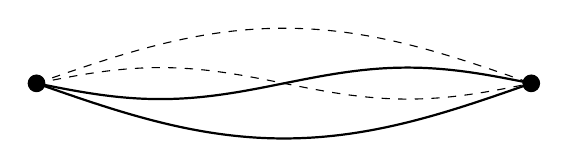
\begin{tikzpicture}[
    tl/.style = {% tick labels
        fill=white, inner sep=1pt, font=\scriptsize,
                },                        ]
    
      \draw[dashed,draw=black,
          domain=-0:6.283,samples=300,variable=\x] 
          plot (\x,{0.7 * sin(deg{\x}/2)});
      \draw[thick,draw=black,
          domain=0:6.283,samples=300,variable=\x] 
      plot (\x,{0.7 * sin(deg{-1 * \x}/2)});
      
      \draw[dashed,draw=black,
          domain=-0:6.283,samples=300,variable=\x] 
          plot (\x,{0.2 * sin(deg{\x})});
      \draw[thick,draw=black,
          domain=0:6.283,samples=300,variable=\x] 
          plot (\x,{0.2 * sin(deg{-1 * \x})});
    
     \filldraw[black] (0, 0)  circle(3pt);
     \filldraw[black] (6.283, 0)  circle(3pt);
    
    \end{tikzpicture}
    
\end{center}
The next overtone has two still points --- it divides the string into
three parts.  The outer parts are up, while the inner part is
down. Its frequency is three times the fundamental frequency.

\begin{center}
    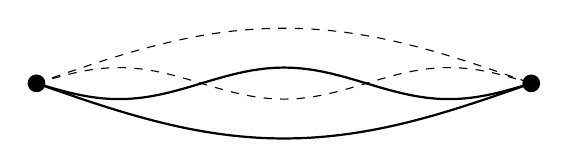
\begin{tikzpicture}[
    tl/.style = {% tick labels
        fill=white, inner sep=1pt, font=\scriptsize,
                },                        ]
    
      \draw[dashed,draw=black,
          domain=-0:6.283,samples=300,variable=\x] 
          plot (\x,{0.7 * sin(deg{\x}/2)});
      \draw[thick,draw=black,
          domain=0:6.283,samples=300,variable=\x] 
      plot (\x,{0.7 * sin(deg{-1 * \x}/2)});
      
      \draw[dashed,draw=black,
          domain=-0:6.283,samples=300,variable=\x] 
          plot (\x,{0.2 * sin(1.5 * deg{\x})});
      \draw[thick,draw=black,
          domain=0:6.283,samples=300,variable=\x] 
          plot (\x,{0.2 * sin(1.5 * deg{-1 * \x})});
    
     \filldraw[black] (0, 0)  circle(3pt);
     \filldraw[black] (6.283, 0)  circle(3pt);
    
    \end{tikzpicture}
    
\end{center}
And so on. 4 times the fundamental, 5 times the fundamental, etc.

In general, tones with many overtones tend to sound bright. Tones
with just the fundamental sound thin.

Humans can generally hear frequencies from 20Hz to 20,000Hz (or
20kHz).  Young people tend to be able to hear very high sounds better
than older people.

Dogs can generally hear sounds from about 65 Hz to 45 kHz, which is why a
dog whistle is silent to you but not to your dog.

\begin{Exercise}[title={A perfect fifth}, label=sound_fifth]
A string vibrates at 220 Hz. What frequency is a perfect fifth above it
(ratio $3:2$)? How does that compare with going up 7 half steps?
\end{Exercise}
\begin{Answer}[ref=sound_fifth]
A perfect fifth: $220 \times \frac{3}{2} = 330$ Hz. Seven half steps:
$220 \times 2^{7/12} \approx 329.63$ Hz. They are very close but not
identical. Modern instruments tune all twelve half steps equally (called
\emph{equal temperament}), so their fifths are very slightly flat.
\end{Answer}

\section{Making waves in Python}

Let us make a sine wave and add some overtones to it.  Create a file named \filename{harmonics.py}.

\begin{minted}{python}
import matplotlib.pyplot as plt
import math

# Constants: frequency and amplitude
fundamental_freq = 440.0 # A = 440 Hz
fundamental_amp = 2.0

# Up an octave
first_freq = fundamental_freq * 2.0 # Hz
first_amp = fundamental_amp * 0.5

# Up a fifth more
second_freq = fundamental_freq * 3.0 # Hz
second_amp = fundamental_amp * 0.4

# How much time to show
max_time = 0.0092 # seconds

# Calculate the values 100,000 times per second
time_step = 0.00001 # seconds

# Initialize 
time = 0.0
times = []
totals = []
fundamentals = []
firsts = []
seconds = []

while time <= max_time:
    # Store the time
    times.append(time)
    
    # Compute value each harmonic
    fundamental = fundamental_amp * math.sin(2.0 * math.pi * fundamental_freq * time)
    first = first_amp * math.sin(2.0 * math.pi * first_freq * time)
    second = second_amp * math.sin(2.0 * math.pi * second_freq * time)

    # Sum them up
    total = fundamental + first + second

    # Store the values
    fundamentals.append(fundamental)
    firsts.append(first)
    seconds.append(second)
    totals.append(total)

    # Increment time
    time += time_step

# Plot the data
fig, ax = plt.subplots(2, 1)

# Show each component
ax[0].plot(times, fundamentals, label="440 Hz")
ax[0].plot(times, firsts, label="880 Hz")
ax[0].plot(times, seconds, label="1320 Hz")
ax[0].legend()

# Show the totals
ax[1].plot(times, totals)
ax[1].set_xlabel("Time (s)")

plt.show()
\end{minted}

When you run it, you should see a plot of all three sine waves and another plot of their sum:
\begin{figure}[H]
    \centering
    \includegraphics[width=0.9\linewidth]{harmonicspy.png}
    \caption{The output of harmonics.py}
    \label{fig:harmonicspy}
\end{figure}

\subsection{Making a sound file}

The graph is pretty to look at, but let us make a file that we can listen to.

The WAV audio file format is supported on pretty much any device, and
a library for writing WAV files comes with Python. Let us write some
sine waves and some noise into a WAV file.

Create a file called \filename{soundmaker.py}

\begin{minted}{python}
import wave
import math
import random

# Constants
frame_rate = 16000 # samples per second
duration_per = 0.3 # seconds per sound
frequencies = [220, 440, 880, 392] # Hz
amplitudes = [20, 125]
baseline = 127 # Values will be between 0 and 255, so 127 is the baseline
samples_per = int(frame_rate * duration_per) # number of samples per sound

# Open a file
wave_writer = wave.open('sound.wav', 'wb')

# Not stereo, just one channel
wave_writer.setnchannels(1)

# 1 byte audio means everything is in the range 0 to 255
wave_writer.setsampwidth(1)

# Set the frame rate
wave_writer.setframerate(frame_rate)

# Loop over the amplitudes and frequencies
for amplitude in amplitudes:
    for frequency in frequencies:
        time = 0.0
        # Write a sine wave
        for sample in range(samples_per):
            s = baseline + int(amplitude * math.sin(2.0 * math.pi * frequency * time))
            wave_writer.writeframes(bytes([s]))
            time += 1.0 / frame_rate
            
        # Write some noise after each sine wave
        for sample in range(samples_per):
            s = baseline + random.randint(0, 15)
            wave_writer.writeframes(bytes([s]))
            
# Close the file
wave_writer.close()
\end{minted}

When you run it, it creates \filename{sound.wav}, with four tones played
quietly and then the same four played loudly. Each tone is followed by a
burst of hiss. Open it in any audio player.

Notice how the tones are made: 16,000 times per second, the program
computes the height of a sine wave and writes it as one number between 0
and 255. That is all digital audio is: a long list of numbers that tell a
speaker where to be.

\begin{Exercise}[title={One Octave Down}, label=sound2]
What is the frequency of the note one octave below $220$ Hz?
\end{Exercise}
\begin{Answer}[ref=sound2]
Half of $220$ Hz, which is $110$ Hz.
\end{Answer}
